\documentclass[border = 1.5cm]{standalone}
%%%% packages
\usepackage{tikz}
\usetikzlibrary{trees, arrows, shapes.geometric} % TikZ libraries
%%%% layers
\pgfdeclarelayer{bg1}    % declare background layer
\pgfdeclarelayer{bg2}
\pgfsetlayers{bg2,bg1,main}  % set the order of the layers (main is the standard layer)

%%%% styles
\tikzset{
	every rectangle node/.style = {draw=black,thick},
	io/.style = {rectangle, minimum width = 4cm, minimum height = 3cm, text centered, draw = black, fill = blue!10},
	main/.style = {rectangle, rounded corners, minimum width = 3cm, text centered, fill = purple!30},
	ids/.style = {diamond, minimum width = 3cm, minimum height = 2cm, text centered, draw = black, fill = green!30},
	res/.style = {rectangle, rounded corners, minimum width = 2cm, minimum height = 1cm, text centered, draw = black, fill = blue!30},
	resvariables/.style = {rectangle, minimum width = 2cm, minimum height = 1cm, text centered, draw = black},
	steps/.style = {rectangle, minimum width = 1cm, text centered, fill = yellow},
	txtfield/.style = {rectangle, rounded corners, text width = 3cm, minimum height = 6cm},
	arrow/.style = {->, > = stealth, draw = black, color = gray!80, shorten > = 2pt, line width = 3pt}
}


\begin{document}
	
	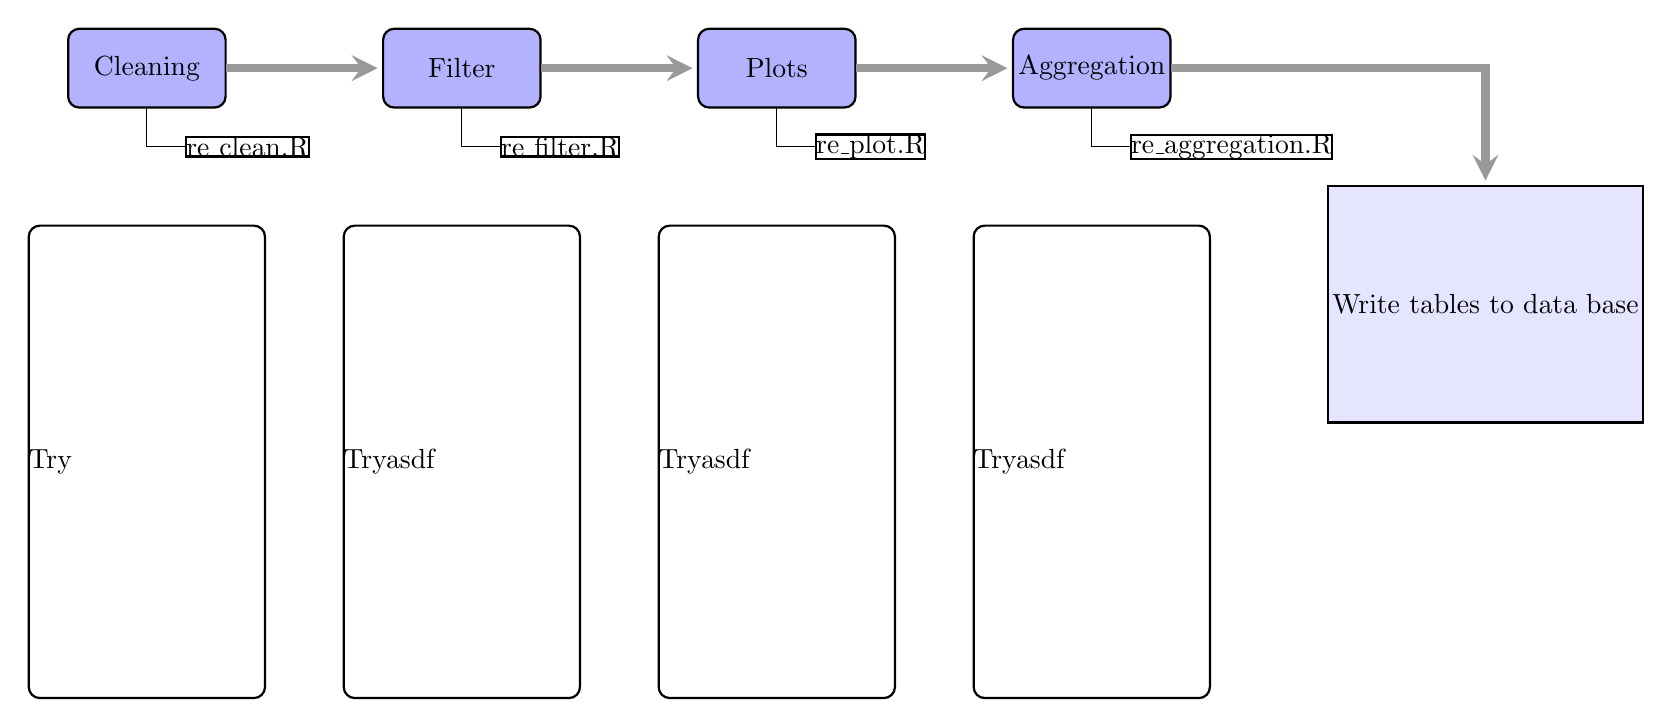
\begin{tikzpicture}[
	grow via three points={one child at (0.5,-1) and
		two children at (0.5,-1) and (0.5,-1.7)},
	edge from parent path={(\tikzparentnode.south) |- (\tikzchildnode.west)},
	anchor = west, inner sep = 0pt, outer sep = 0pt
	]
	
	%\draw[thick] (current page.south west) rectangle (current page.north east); % debuging
	
	%% nodes	
	\node (clean) [res] at (0cm,0cm) {Cleaning}
	child { node { re\_clean.R} };
	\node (filter) [res, right of = clean, xshift = 3cm] {Filter}
	child { node { re\_filter.R} };
	\node (plot) [res, right of = filter, xshift = 3cm] {Plots}
	child { node { re\_plot.R} };
	\node (agg) [res, right of = plot, xshift = 3cm] {Aggregation}
	child { node { re\_aggregation.R} };
	
	\node (write) [io, right of = agg, xshift = 4cm, yshift = -3cm] {Write tables to data base};
	
	%% text fields
	%\node (txtclean2) [txtfield, below of = clean, yshift = -4cm] {Test2};
	\node (txtclean2) [txtfield, below of = clean, yshift = -4cm] {Try};
	\node (txtclean2) [txtfield, below of = filter, yshift = -4cm] {Tryasdf};
	\node (txtclean2) [txtfield, below of = plot, yshift = -4cm] {Tryasdf};
	\node (txtclean2) [txtfield, below of = agg, yshift = -4cm] {Tryasdf};
	
	%% arrows
	\draw [arrow] (clean) -- (filter);
	\draw [arrow] (filter) -- (plot);
	\draw [arrow] (plot) -- (agg);
	\draw [arrow, to path={-| (\tikztotarget)}] (agg) edge (write.north);
	
	
	%% cleaning and filter steps
	
	
	\iffalse
	\node (solub) [steps, below of = clean, yshift = -2cm] {Solubility check};
	\node (substtype) [steps, below of = clean, yshift = -4cm] {Substance-type: F, AI, U, T};
	
	\node (habitat) [steps, right of = solub, xshift = 7cm] {Habitat: Marine, Brackish, Freshwater, Terrestrial};
	\node (region) [steps, right of = solub, xshift = 7cm, yshift = -2cm] {Regions: Americas, Africa, Freshwater, Terrestrial};
	\node (duration) [steps, right of = solub, xshift = 7cm, yshift = -4cm] {Tests between 22 and 338h};
	\node (taxagroups) [steps, right of = solub, xshift = 7cm, yshift = -6cm] {};
	
	\node (agg1) [steps, right of = solub, xshift = 7cm, yshift = -6cm] {by casnr, taxon and duration};
	
	%% arrows
	\draw [->, dashed] (-5,8) -- (clean);
	
	%% boxes
	\draw [dashed] (1,6) rectangle (3,-11);
	\draw [dashed] (4,5) rectangle (7,-11);
	\draw [dashed] (9,5) rectangle (11,-11);
	\draw [dashed] (14,5) rectangle (15,-11);
	\fi
	\end{tikzpicture}
\end{document}

